\section{Dasar Teori}

\textit{Block cipher} merupakan algoritma enkripsi simetris yang mengamankan data dengan membagi pesan ke dalam blok-blok bit berukuran tetap (biasanya 64 bit, 128 bit, dsb) dan mengolahnya melalui beberapa putaran transformasi. Untuk menjamin keamanannya, rancangan algoritma harus memenuhi prinsip \textit{confusion} dan \textit{diffusion} dengan tetap menggunakan operasi yang sederhana seperti substitusi dan transposisi.

\begin{figure}[h]
    \centering
    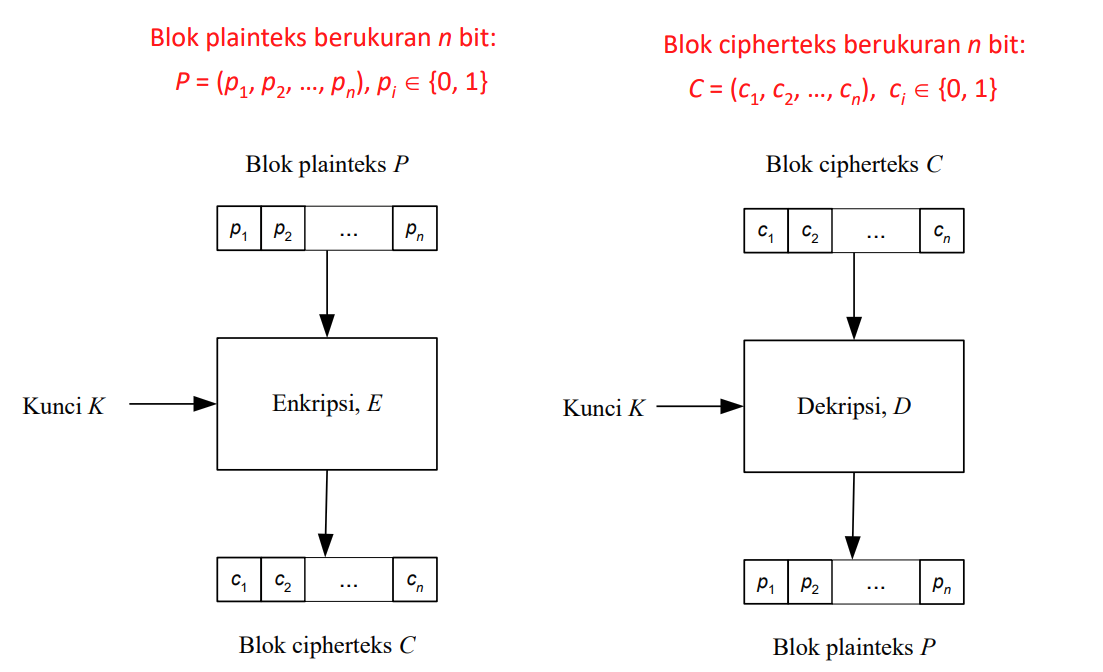
\includegraphics[width=0.5\textwidth]{images/block-cipher.png}
    \caption{Ilustrasi Block Cipher}
    \label{fig:block_cipher}
\end{figure}

\subsection{\textit{Confusion} dan \textit{Diffusion}}
Menurut the GOAT Claude Shannon, dua konsep ini adalah syarat sebuah cipher yang baik. \textit{Confusion} mengaburkan hubungan antara kunci dan teks sandi, sedangkan \textit{diffusion} menyebarkan pengaruh setiap bit dari plainteks ke banyak bit cipherteks. Pada praktiknya, \textit{confusion} dicapai dengan operasi nonlinier seperti S-box, sedangkan \textit{diffusion} dicapai dengan operasi linier yang mencampur dan memindahkan bit, seperti permutasi. Kedua operasi tersebut diulang dalam beberapa putaran sehingga efeknya saling memperkuat.

\subsection{Jaringan Feistel}
Jaringan Feistel adalah struktur yang digunakan dalam banyak algoritma block cipher, termasuk DES. Struktur ini membagi blok input menjadi dua bagian, biasanya disebut sebagai \textit{left} dan \textit{right}. Setiap putaran dari jaringan Feistel melibatkan fungsi \textit{round} yang diterapkan pada salah satu bagian, kemudian hasilnya digabungkan dengan bagian lainnya menggunakan operasi XOR. Proses ini diulang selama beberapa putaran, dan pada akhir proses, kedua bagian digabungkan kembali untuk membentuk blok output. Salah satu keuntungan utama dari jaringan Feistel adalah bahwa dekripsi dapat dilakukan dengan menggunakan algoritma yang sama dengan enkripsi, hanya dengan membalik urutan kunci putaran.

Keuntungan lain dari jaringan Feistel adalah fungsi \textit{round} tidak perlu dapat dibalik, karena dekripsi cukup menghitung ulang fungsi tersebut lalu membatalkan operasi XOR. Apabila kedua bagian blok berukuran tidak sama, strukturnya disebut jaringan Feistel tak seimbang (\textit{unbalanced Feistel network}). Selain XOR, penggabungan hasil fungsi \textit{round} juga dapat menggunakan operasi lain yang memiliki invers, misalnya penjumlahan modulo $2^n$, sehingga dekripsi menggunakan pengurangan modulo $2^n$.

\begin{figure}[htb!]
    \centering
    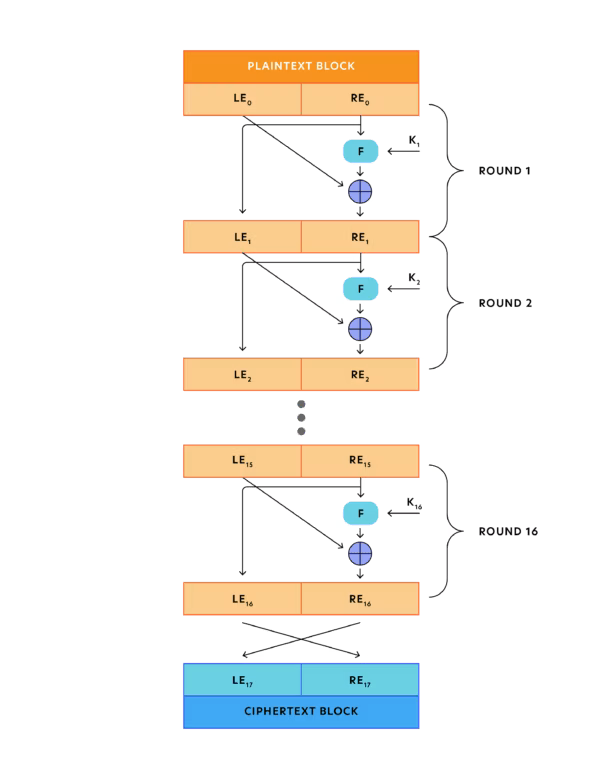
\includegraphics[width=0.5\textwidth]{images/feistel.png}
    \caption{Struktur Jaringan Feistel}
    \label{fig:feistel}
\end{figure}

\pagebreak
\subsection{Substitusi dan Permutasi}
Substitusi adalah proses mengganti satu simbol dengan simbol lain, sedangkan permutasi adalah proses mengatur ulang urutan simbol-simbol tersebut. Keduanya merupakan operasi dasar dalam enkripsi dan digunakan untuk mencapai prinsip \textit{confusion} dan \textit{diffusion}. 
Kombinasi dari substitusi dan permutasi membentuk dasar dari banyak algoritma block cipher modern, termasuk AES. Dalam AES, blok data diolah melalui beberapa putaran yang melibatkan substitusi byte menggunakan S-box, pergeseran baris, pencampuran kolom, dan penambahan kunci putaran.

Beberapa operasi yang termasuk dalam substitusi dan permutasi adalah \texttt{SubBytes} yang mengganti setiap byte dengan byte lain menggunakan S-box, \texttt{ShiftRows} yang menggeser baris-baris dari blok data, \texttt{MixColumns} yang mencampur kolom-kolom dari blok data, dan \texttt{AddRoundKey} yang menambahkan kunci putaran ke blok data menggunakan operasi XOR.

S-box yang baik bersifat bijektif dan nonlinier. Salah satu cara membangunnya, seperti pada AES, adalah menghitung invers multiplikatif setiap byte di medan Galois $GF(2^8)$, yaitu himpunan polinomial berderajat kurang dari 8 dengan koefisien biner yang dioperasikan modulo sebuah polinomial tak tereduksi berderajat 8. Invers multiplikatif memberikan nonlinieritas yang tinggi, kemudian hasilnya dikenai transformasi afin untuk menghilangkan struktur aljabar yang terlalu sederhana. Tabel hasil konstruksi ini disimpan sehingga substitusi cukup dilakukan dengan \textit{table lookup}.

\subsection{Operasi Tambahan}
Selain substitusi dan permutasi, \textit{block cipher} umumnya menggunakan operasi tambahan yang sederhana dan dapat dibalik.
\begin{itemize}[noitemsep]
    \item \textbf{Rotasi bit}, yaitu pergeseran sirkular sebanyak $k$ posisi. Inversnya adalah rotasi ke arah berlawanan.
    \item \textbf{Penjumlahan modulo $2^n$}. Operasi ini nonlinier terhadap XOR sehingga menambah \textit{confusion}, dan inversnya adalah pengurangan modulo $2^n$.
    \item \textbf{\textit{Xorshift}}, yaitu operasi $x \leftarrow x \oplus (x \ll k)$ atau $x \leftarrow x \oplus (x \gg k)$ yang diperkenalkan oleh Marsaglia pada pembangkit bilangan acak. Operasi ini menyebarkan satu bit ke beberapa posisi dan dapat dibalik karena sebagian bit tidak berubah dan dapat dipulihkan secara bertahap.
    \item \textbf{Kompresi dan ekspansi bit}, yaitu pemetaan antara ukuran bit yang berbeda. Kompresi tidak dapat dibalik, sehingga hanya aman digunakan sebagai \textit{mask} atau di dalam fungsi \textit{round} Feistel.
\end{itemize}

\subsection{Fungsi Kompresi SHA-256}
SHA-256 adalah fungsi hash yang memproses pesan dalam blok 512 bit. Setiap blok diperluas menjadi 64 kata 32-bit $W_t$ (\textit{message schedule}), kemudian diolah oleh fungsi kompresi selama 64 putaran yang memperbarui delapan variabel kerja $a, b, \ldots, h$. Setiap putaran menggunakan rotasi, pergeseran, penjumlahan modulo $2^{32}$, fungsi nonlinier $Ch$ dan $Maj$, serta konstanta putaran $K_t$. Fungsi kompresi ini dirancang agar perubahan kecil pada masukan mengubah keluaran secara acak dan sulit dibalik, sehingga cocok digunakan sebagai fungsi \textit{round} pada jaringan Feistel. Apabila konstanta $K_t$ diturunkan dari kunci, fungsi ini berperan sebagai fungsi berkunci (\textit{keyed function}).

\subsection{Penjadwalan Kunci}
Penjadwalan kunci (\textit{key schedule}) membangkitkan kunci putaran yang berbeda untuk setiap putaran dari kunci utama. Konstanta putaran yang berbeda di setiap putaran diperlukan agar setiap putaran tidak identik, karena putaran yang identik membuat cipher rentan terhadap \textit{slide attack}. Apabila satu putaran membutuhkan beberapa kunci, kunci-kunci tersebut dapat diturunkan dari kunci putaran yang sama menggunakan konstanta yang berbeda. Teknik ini disebut pemisahan domain (\textit{domain separation}) dan mencegah dua komponen menggunakan kunci yang identik.

\subsection{Mode Operasi dan \textit{Padding}}
\textit{Block cipher} hanya mengenkripsi satu blok berukuran tetap, sehingga pesan yang lebih panjang diproses menggunakan mode operasi. Mode selain ECB menggunakan \textit{Initialization Vector} (IV) atau \textit{counter} agar plainteks yang sama menghasilkan cipherteks yang berbeda. 

\begin{table}[H]
    \centering
    \small
    \caption{Ringkasan mode operasi \textit{block cipher}}
    \label{tab:mode_operasi}
    \begin{tabularx}{\textwidth}{@{}l >{\raggedright\arraybackslash}X >{\raggedright\arraybackslash}X@{}}
        \toprule
        \textbf{Mode} & \textbf{Enkripsi blok ke-$i$} & \textbf{Keterangan} \\
        \midrule
        ECB & $C_i = E_K(P_i)$ & Tanpa IV; blok plainteks yang sama menghasilkan blok cipherteks yang sama. \\
        CBC & $C_i = E_K(P_i \oplus C_{i-1})$, $C_0 = IV$ & Setiap blok bergantung pada blok sebelumnya. \\
        CFB & $C_i = P_i \oplus E_K(C_{i-1})$, $C_0 = IV$ & Bekerja seperti \textit{stream cipher}; hanya membutuhkan $E_K$. \\
        OFB & $O_i = E_K(O_{i-1})$, $O_0 = IV$; $C_i = P_i \oplus O_i$ & \textit{Keystream} tidak bergantung pada plainteks. \\
        CTR & $C_i = P_i \oplus E_K(\textit{ctr} + i)$ & Setiap blok dapat diproses secara independen. \\
        \bottomrule
    \end{tabularx}
\end{table}